\documentclass{llncs}
\usepackage{fancyhdr, tabularx, verbatim, epsfig}
\usepackage{amssymb,psboxit}
\usepackage{rotating}
\usepackage{tabularx}
\newcommand{\amesos}{{\sc Amesos}}

\newtheorem{interface}{Interface}[section]

\begin{document}

\pagestyle{headings} 
\mainmatter              % start of the contributions

\title{\amesos: A Set of General Interfaces to Sparse Direct Solver Libraries}
%
\titlerunning{Interfaces to Direct Solvers}  % abbreviated title (for running head)
%                                     also used for the TOC unless
%                                     \toctitle is used
%
\author{Marzio Sala\inst{1} \and Ken Stanley\inst{2} \and
Michael A. Heroux\inst{3}}
%
\authorrunning{Marzio Sala et al.}   % abbreviated author list (for running head)
%
%%%% modified list of authors for the TOC (add the affiliations)
\tocauthor{Marzio Sala (ETH Zurich),
Ken Stanley (Oberlin College),
Michael A. Heroux (Sandia National Laboratories)}
%
\institute{Department of Computer Science, ETH Zurich, CH-8092 Zurich\\
\email{marzio@inf.ethz.ch}
\and
Department of Computer Science, Oberlin College, Oberlin, Ohio, USA \\
\and
PO Box 5800 MS 1110, Albuquerque, NM 87185-1110
\footnote{
ASCI program and the DOE Office of Science MICS program at Sandia
National Laboratory.  Sandia is a multiprogram laboratory operated by
Sandia Corporation, a Lockheed Martin Company, for the United States
Department of Energy's National Nuclear Security Administration under
contract DE-AC04-94AL85000.}
}

\maketitle              % typeset the title of the contribution

\begin{abstract}
We present the \amesos\ project, which aims to define a set of general,
flexible, consistent, reusable and efficient interfaces to direct solution
software libraries for systems of linear equations on both serial and
distributed memory architectures. \amesos is composed by a collection of pure
virtual classes, as well as several concrete implementations in the C++
language. These classes allow to access the linear system matrix and vector
elements and their distribution, and control the solution of the linear
system. We report numerical results that show that the overhead induced by the
object-oriented design is negligible under typical conditions of usage. We
include examples of applications, and we comment on the advantages and
limitations of the approach.
\end{abstract}

% --------------------------------------------------------------------------- %
\section{Introduction}
\label{sec:introduction}
% --------------------------------------------------------------------------- %

This paper describes the design and the implementation of 
interfaces to serial and parallel direct solution libraries for
linear systems of type
\begin{equation}
  \label{eq:linear_system}
  A x = b,
\end{equation}
where $A \in \mathbb{R}^{n \times n}$ is a real and sparse square matrix, 
  and $x, b \in \mathbb{R}^{n}$ are the solution and
the right-hand side vectors, respectively. 

Generally speaking,
a direct solution algorithm for (\ref{eq:linear_system}) is any 
technique that computes three matrices, $L$, $D$ and $U$, such that
$P\, A\, Q = L \, D \, U$, where $P$ and $Q$ are permutation matrices
and the linear systems with matrices $L$, $D$ and $U$ are
easy to solve.
The process of computing these three matrices is called {\sl
  factorization}. Generally, $L$ is a lower triangular matrix, $U$ is an
upper triangular matrix, $D$ is a diagonal matrix 
(or possibly the identity matrix), and the algorithm adopted for their
computation is some variant of the Gaussian elimination method.

The point of view of this paper is that of application developers, interested
in {\sl using} direct solver libraries for a specific problem. As such, we
will not consider their {\sl development}; instead, we suppose that software
libraries offering algorithms for the direct solution of
(\ref{eq:linear_system}) are already available. The objective is {\sl
interfacing} one or more of these libraries with the application code under
study.  This usually involves the following steps. First, a library is chosen
because of its robustness, performances in terms of CPU time and memory,
documentation, usage, availability. Then, an interface between the application
code and the library is written, and this usually requires storing the linear
system matrix $A$ using the storage format required by the library. Finally, 
the calling sequence is hard-wired in the final application code.
The outlined process is typically repeated every time a new application is
developed, and every time a new solver is under consideration. 

\smallskip

Note that,
for distributed sparse solvers, no
``gold standard'' exists. Therefore, application developers aiming to solve
(\ref{eq:linear_system}) generally have to look for a suitable
library that meets their needs. The choice is affected by several criteria,
likeseveral criteria,
like the easiness of
usage, availability, the quality of documentation and support, and of course
the set of capabilities, the solution time, and the memory usage.
The relative importance of these aspects is usually subjective. For
relatively simple problems, the performance is usually the key point, followed
by memory usage. For complicated problems, and especially in industrial
applications, reliability is of paramount importance.

Once a library has been chosen, the application developers have to write a
custom-made interface between the selected library and the application. This
usually requires storing the linear system matrix $A$ using the storage format
required by the library, then calling the correct sequence of instructions to
factor the matrix and solve the linear system.  In our opinion, the approach
is sub-optimal for both application and library developers because it:
\begin{enumerate}

\item
{\bf Offers partial coverage}. Writing a custom-made interface means
that only the targeted library will be used. This is inconvenient
because of the already mentioned difficulty to choose {\it a-priori}
the best library for a given application. In some cases, a
theoretical analysis of the problem at hand can suggest the right
algorithm. Alternatively, one can consider numerical comparisons on
test matrices available in the literature.
Often, however, one has to validate a given library on the
application, architecture, and data set of interest, and this can be
done only if the interface is already available;

\item
{\bf Produces maintenance problems}. Including the interfaces within
the application code requires the application developers to
manipulate the matrix format, the memory management, the calling
conventions, and others, that can vary from one library to the
following. Although not necessary difficult, these activities are
usually time-consuming;

\item
{\bf Delays the usage of new libraries}. Large application codes
usually have a long life.  The sheer size of the codes and a natural
reluctance to change successful projects discourage any effort of
rewriting unless absolutely necessary. Since a new library (or a new
version of a given library) may require a new matrix format or
distribution, or new calling conventions, application developers may
simply decide to continue using the interface already developed.
\end{enumerate}

In this paper, we present a software project, called \amesos\, which aims to
address these problems by using object-oriented (OO) design and programming.
\amesos\ is composed by a set of clean, consistent and easy-to-use interfaces
between the application and the direct solver libraries.  Each interface takes
care of dealing with the direct solver library, in a manner that is
transparent to the application developers, and automatically manages matrix
formats, data layout, and calling conventions. \smallskip

\smallskip

The paper is organized as follows. Section~\ref{sec:design} describes the
requirements and the design of the \amesos\ project. The basic classes are
outlined in Section~\ref{sec:basic}, and the list of supported solvers is
given in Section~\ref{sec:supported}.  Section~\ref{sec:numerical} reports an
example of usage and some numerical results that quantify the overhead
required by the generality of the approach.  Finally,
section~\ref{sec:conclusions} outlines the conclusions.

%-----------------------------------------------------------------------------
\section{Project Design}
\label{sec:design}
%-----------------------------------------------------------------------------

The \amesos\ design is based on the following requirements:
\begin{enumerate}
%
\item {\bf Simplicity of usage}. Solving linear system (\ref{eq:linear_system}) in a language
like MATLAB is very easy, i.e.~one just writes \verb!x = A \ b!. It should not be much
more difficult in a production code;
%
\item {\bf Flexibility}. More than one algorithm/library must be available,
  for both serial and parallel architectures;
%
\item {\bf Efficiency}. The overhead due to the framework must be minimal.
\end{enumerate}

The basic ideas of this design are indeed quite old, and can be traced back to
almost 30 years ago~\cite{duff79performance,george79design}. More recently,
  articles~\cite{george99object,dobrian99design} discussed the usage of
  abstract interfaces and OO design for the direct solution of sparse linear
  systems.  We extend these ideas by abstracting the concepts to
a higher level, and making the interfaces independent of the
supported libraries. The interfaces are presented and implemented as
a set of C++ classes using several well-known design
patterns. C++ supports object-oriented
programming, and it is relatively easy to interface FORTRAN77,
FORTRAN90 and C libraries with C++ code. The C++ language supports
abstraction through classes, inheritance and polymorphism. For
application developers, abstraction is important because it brings
simplicity, by allowing components with a minimal interface. It also
ensures flexibility because it decouples the different algorithmic
phases from the data structures. Finally, abstraction allows
extensibility in the sense that new (yet to be developed) libraries
can be easily added, at almost no cost to the application developer.
Another candidate language could have been FORTRAN90, but it does
not have inheritance and polymorphism.

Regarding the parallel computing mode, we consider parallel
architectures with distributed memory, and we suppose that the
message passing interface MPI is adopted. This
approach is the de-facto standard in scientific computing. As a result,
the presented design can be easily interfaced with the
aforementioned projects.

%-----------------------------------------------------------------------------
\section{Basic Classes}
\label{sec:basic}
%-----------------------------------------------------------------------------

The key point of our design is to manage all direct solver libraries by a
workflow structured as follows:
\begin{enumerate}
\item Definition of the sparsity pattern of the linear system matrix;
\item Computation of the symbolic factorization, which includes
preordering and analysis. The
symbolic factorization refers to all operations that can be performed by
accessing the matrix structure only (without touching the values of the matrix entries);
\item Definition of the values of the linear system matrix;
\item Computation of the numeric factorization, that is, the computation
of the entries of the factored terms;
\item Definition of the right-hand side $b$;
\item Solution of the linear system, that is, computation of $x$.
\end{enumerate}
Steps 1, 3 and 5 are application-dependent and will not be discussed
here; instead, our aim is to standardized steps 2, 4 and
6  by adding an intermediate layer between the application and
the direct solver libraries.  The design discussed below uses
several common design patterns~\cite{Gamma}.  The first is the
\textit{Builder Pattern}, by which we define an abstract class whose
methods are steps 2, 4 and 6.  Because each of these steps could in
principle be replaced with an alternate algorithm, our design also
represents the \textit{Strategy Pattern}. Finally, we use the
\textit{Factory Pattern} as a means of selecting a specific concrete
solver instance by use of a string argument.

Presently we introduce a set of abstract classes, which will be used
to define interfaces to the data layout of distributed objects,
vectors, matrices, linear system, and the solver. The design is
reported here as a set of C++ classes, but the concepts are more
general and the discussion is largely language-independent.

Our design is based on a set of C++ pure virtual classes, which will be
used to define interfaces to the data layout of distributed objects, 
vectors, matrices, linear system, and the solver. These classes are:
a {\tt Map} class that specifies the layout of matrix rows;
a {\tt Vector} class that defines distributed vectors;
a {\tt Matrix} class which offers a standard calling sequence to access
matrix elements. We suppose that each matrix row is assigned to exactly one
processor, and it is easy to access all nonzero elements
of any locally owned row by calling a {\tt GetRow()} method which returns the
nonzero indices and values for the specified (local) row;
a {\tt LinearProblem} class which contains the linear system matrix, the
solution and the right-hand side vectors;
a {\tt Solver} class that manages the underlying solver library. 

The pure virtual class {\tt Solver} deserves more details. This class contains
the following methods:
\begin{itemize}
\item
\verb!void SetLinearProblem()! sets the linear problem
to solve;
\item
\verb!void SetParameters(List)! specifies all the parameters for the solver by
using a generic container (hash table);
\item
\verb!int SymbolicFactorization()! performs the symbolic factorization, that
is, all the operations that do only require the matrix graph and not the
actual matrix values;
\item
\verb!int NumericFactorization()! performs the numeric factorization, that
is, it computes the matrices $L$, $D$ and $U$ by accessing the matrix values.
Both the solution and the right-hand side vectors are not required in this phase;
\item
\verb!int Solve()! solves the linear system. This phase requires the
solution and the right-hand side vectors.
\end{itemize}

The design is organized
as follows: each interface is defined by a class, derived from the
pure virtual {\tt Solver} class, and it internally allocates and manages all
the objects required by the underlying solver. This insulates the user from
lower-level details. 

%------------------------------------------------------------------------- 
\section{Supported Libraries}
\label{sec:supported}
%------------------------------------------------------------------------- 

\amesos\ offers interfaces to the following direct solvers: LAPACK, ScaLAPACK,
KLU\footnote{The sources of KLU are distributed within \amesos.}
\cite{davis05klu}, UMFPACK~\cite{umfpack-home-page}, SuperLU and
SuperLU\_DIST~\cite{superlu-manual} DSCPACK~\cite{dscpack-manual},
MUMPS~\cite{mumps-manual}, TAUCS~\cite{irony04parallel}, and
PARDISO~\cite{oskl:04-etna,sg:04-fgcs}. Other interfaces are under
development.

\amesos\ takes advantage of the {\sc Epetra} package~\cite{Epetra-Ref-Guide}
to specify the {\tt Map, Vector, Matrix} and {\tt LinearProblem} interfaces.
The Standard Template Library (STL) is used to increase performances
whenever possible.

To increase portability, \amesos\ is configured using
Autoconf and Automake; each
interface can be enabled or disabled at configure time. Users can
take advantage of the bug-tracking tool Bugzilla to
provide feedback or request improvements. \amesos\ can be downloaded as part of
the Trilinos framework at the web
page
\verb!http://software.sandia.gov/trilinos/packages/amesos!. More details on
the usage of \amesos\ can found in~\cite{Amesos-Reference-Guide} and the
on-line documentation, while the
design is presented in great details in \cite{sala06design}.

%------------------------------------------------------------------------- 
\section{Example of Usage and Numerical Results}
\label{sec:numerical}
%------------------------------------------------------------------------- 

An example of usage of \amesos\ is reported in Figure~\ref{fig:example}.
Although this particular example requires MPI, \amesos\ can be compiled with
or without support for MPI.  (Clearly, distributed solvers are available only
when compiled with MPI support.) The only \amesos\ include file is
\verb!Amesos.h!, which does not include the header files of the supported
library.  The required interface is specified by the string variable
\verb!SolverType!, and is created by using the factory class \verb!Amesos!.
Factory classes are a programming tool that implements a sort of ``virtual
constructor,'' in the sense that one can instantiate a derived (concrete)
object while still working with abstract data types. The example reported in
Figure~\ref{fig:example} adopts UMFPACK as a solver; however by using the
factory class, other interfaces can be created by simply changing the
parameter {\tt SolverType}. Note that the supported solver can be serial or
parallel, dense or sparse: the user code still remains the same, except for
the name of the solver; \amesos\ will take care of data redistribution if
required by the selected solver.

\begin{figure}
\begin{center}
\begin{tabular}{| p{12cm} | }
\hline
 \\ $\,$
\begin{minipage}{11.8cm}
\begin{verbatim}
#include "Amesos.h"
#include "mpi.h"
#include "Epetra_MpiComm.h"
...

int main(int argc, char *argv[])
{
  MPI_Init(&argc, &argv);
  Epetra_MpiComm Comm(MPI_COMM_WORLD);

  Epetra_Map* Map = <create map here, Interface 3.1>;
  Epetra_MultiVector* x = <create solution vector here, Interface 3.2>;
  Epetra_MultiVector* b = <create right-hand side here, Interface 3.2>;
  Epetra_CrsMatrix* A = <create matrix here, Interface 3.3>;

  Epetra_LinearProblem Problem(A, x, b); // Interface 3.4

  Amesos Factory;                  // create a factory class
  string SolverType = "Umfpack";   // selected interface
  Amesos_BaseSolver* Solver;       // generic solver object, Int. 3.5
  Solver = Factory.Create(SolverType, Problem); // create solver

  Teuchos::ParameterList List;     // allocate container for params,
  List.set("PrintTiming", true);   // set one in the container, then
  Solver->SetParameters(List);     // pass the container to the solver

  Solver->SymbolicFactorization(); // symbolic factorization
  Solver->NumericFactorization();  // numeric factorization
  Solver->Solve();                 // linear system solution
  delete Solver;

  MPI_Finalize();
  return(EXIT_SUCCESS);
} // end of main()
\end{verbatim}
\end{minipage} \\
 \\
 \hline
\end{tabular}
\caption{Example of code using \amesos. The code uses the \amesos\ interface to
  UMFPACK to solve the linear system. The creation of the matrix, solution and
    right-hand side are not reported.}
\label{fig:example}
\end{center}
\end{figure}

The example code of Figure~\ref{fig:example} has shown the facility of usage
of \amesos. We now address the effectiveness of the interface.
Figure~\ref{fig:results} reports the percentage of CPU time required by the
\amesos\ interface with respect to the time required by the underlying
library. We have considered the SuperLU and UMFPACK interface for the solution
of all matrices in the FIDAP collection, available
at~\cite{boisvert97matrix}. The matrix sizes range from 27
({\tt FIDAP005}) to 22294 ({\tt FIDAPM11}). All problems are solved using a
1.67 GHz G4 processor with 1024 Mbytes of RAM, running MAC OS X 10.4 and gcc
4.0.0. The table reports the percentage of the CPU time required by the
interface with respect to the time required by the considered solver, and
quantifies the overhead required by \amesos. We have used the default set of
parameters for both solvers.

As expected, for small matrices (for example \verb!FIDAP005! or
\verb!FIDAPM05!, of size 27 and 42, respectively) the overhead is
considerable. When considering bigger matrices ($n > 3000$), then the overhead
is  always below 5\%. All the overhead is spent in converting the matrix from
the abstract matrix format to the format required by the
library, and performing additional safety checks.  Note that this overhead can
indeed be reduced by adding specialized classes, that satisfies the
interface and internally store the matrix in the format required
by a given solver library, then 
perform a {\tt dynamic\_cast} to obtain the already allocated data
structure containing the matrix. This solution is inelegant and requires
knowledge of derived classes in the solver interface, but could greatly
increase performance. 

\begin{figure}
\begin{center}
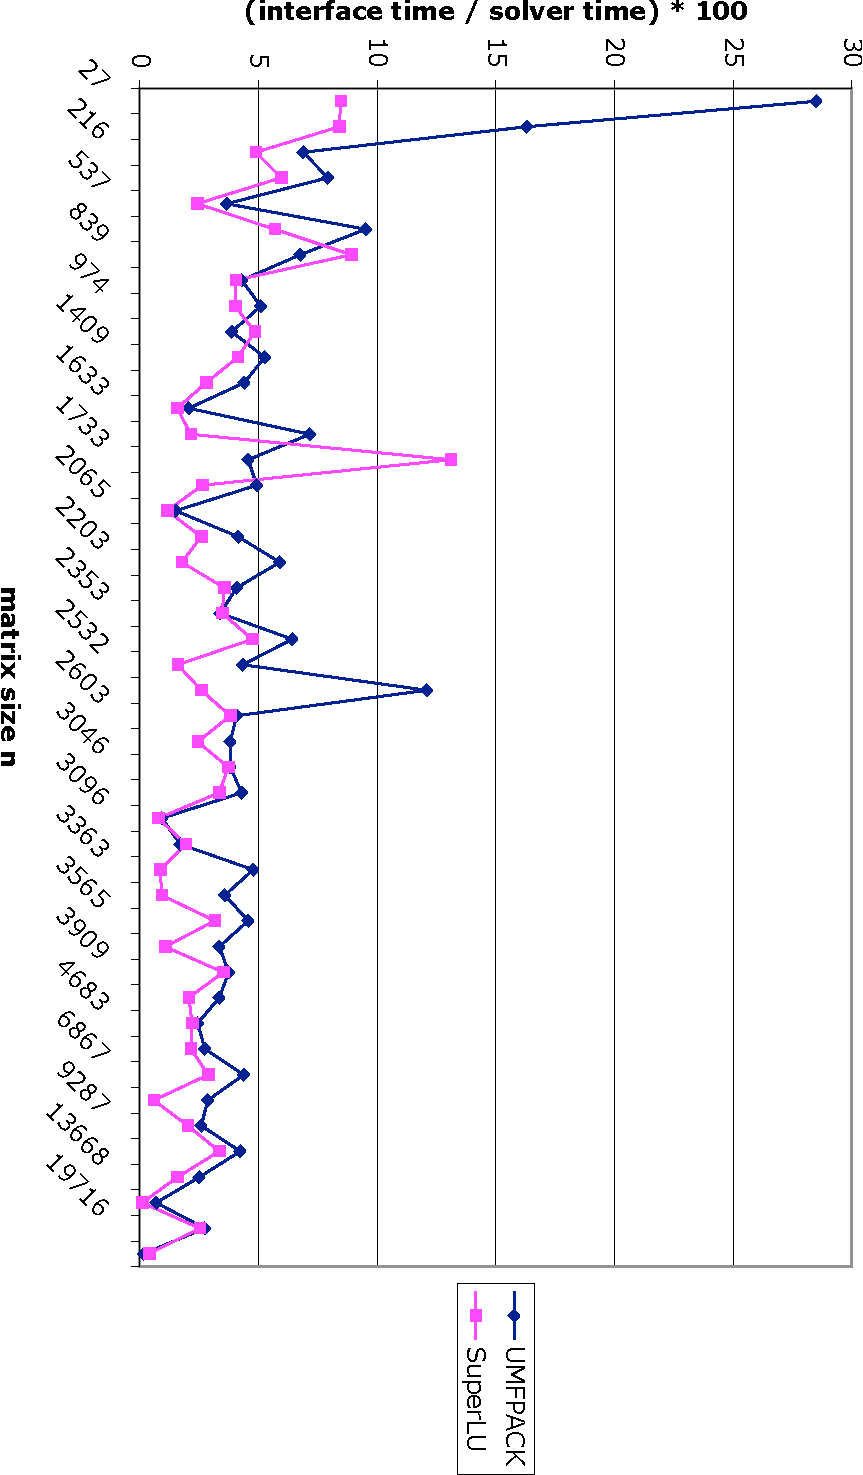
\includegraphics[angle=90,width=12cm]{../AmesosOverview/interface_time.pdf}
\caption{Additional time required by the \amesos\ interface with respect to the
time required by the solver, for different matrices and solvers. $n$
  represents the size of the matrix, and $nnz$ the total number of nonzeros.
The results were obtained on a G4 1.67 GHz with 1 GByte of RAM.}
\label{fig:results}
\end{center}
\end{figure}

%-----------------------------------------------------------------------------
\section{Concluding Remarks}
\label{sec:conclusions}
%-----------------------------------------------------------------------------

In this paper, we have presented the \amesos\ project, which defines a model
to access direct solver libraries. The advantages of this model are the
following:
\begin{itemize}
%
\item The actual data storage format of the linear system matrix becomes largely unimportant.
Each concrete implementation will take care, if necessary, to convert the
input matrix to the required data format. This means that the
application can choose {\sl any} matrix format that can be wrapped by the
abstract matrix interface.
%
\item Issues like diagonal perturbations, dropping, reordering or
fill-reducing algorithms
can be easily introduced within the abstract matrix interface.
For example, a dropping strategy or a modification of the diagonals simply
requires a new \verb!GetMyRow()! method, without touching the actual matrix
storage. Also, reordering techniques can be implemented and tested
independently of the library used to perform the factorization.
%
\item The actual calling sequence required by each library to factor the
matrix and solve the linear system is no longer exposed to the user, who only
has to call methods \verb!SymbolicFactorization()!, \verb!NumericFactorization()! and
\verb!Solve()!.
%
\item Interfaces can be tested more easily because they are all located within
the same library and not spread out into several application codes. The
framework is also quite easy to learn and use, since a basic usage
requires about 20 code lines (see the example of Figure~\ref{fig:example}).
%
\item It is easy to compare different solvers on a given set of problems. The
\amesos\ distribution contains a (working) template that reads a linear system
from file in the popular Harwell/Boeing format~\cite{duff89sparse} and solves it with all the
enabled solvers. Users can easily modify this template to numerically evaluate
the optimal library for {\sl their} problems.
%
\item
The framework can serve users with different levels of expertise, from the
usage of libraries as black-box tools, to a fine-tuning of each library's
parameters.
%
\item
The framework can be easily extended to incorporate libraries for the
resolution of over-determined and under-determined systems. Solving such
systems may involve algorithms other than Gaussian eliminations; nevertheless,
the interfaces will remain almost untouched.
%
\end{itemize}

The generality of the proposed model comes at a price. The presented model has the following
limitations:
\begin{itemize}
\item
Overhead may be introduced when converting or redistributing the
matrix and/or the vectors into the library's format. For very large
matrices, this can constitute a problem especially in terms of
memory consumption, but is often not a first-order concern.
\item
Fine-tuning of solver's parameters can be difficult. Also, we offer no
``intelligent'' way of setting these parameters.  
%
\item There is no standard way to convert MPI communicators defined in C to
MPI communicators defined in FORTRAN90. On some architectures it is difficult
or even impossible to perform such a task. Some hacks may be required.
%
\item
It is almost impossible to support different releases of a given
software library, because function names usually do not change from
one version to the next, making it impossible for the linker to
select the
  appropriate version of the library.
%
\item
Some libraries offer a one-solve routine without storing any data after the
solution is completed; this option is not  supported
by the presented design, but it could be easily added.
%
\item
There are no capabilities to obtain the $L$, $D$ and $U$ factors, or the
reorderings $P$ and $Q$. This is because each supported package uses a
different storage format and distribution. Reordering and scaling can be made
library-independent by working the presented abstract interfaces.
%
\item
Problematic user-package communications. Because of the high-level view, the
code is safer: it is more difficult to make errors or call the solver with the
wrong set of parameters. \amesos\ classes automatically perform safety checks,
      and return an error code when something goes wrong. However,
it is often difficult to abstract the error
messages from all supported libraries and report them in a uniform fashion.
Users still need to consult the library's manual to decode the error messages.
\end{itemize}

Despite these issues, we find that the presented set of interfaces
brings its users the well-known benefits of reusable libraries.
Thanks to their generality, these interfaces (and the corresponding
codes) can be used to easily connect intricate applications with
state-of-the-art linear solver libraries, in a simple and
easy-to-maintain way. From the point of view of application
developers, the small amount of required code makes it very
convenient to adopt a project like \amesos. For linear solver
libraries' developers  writing one interface for their own solver
can help to make it applicable and testable to a vast range of
applications.

One of our goal in the design of \amesos\ was to reduce the intellectual
effort required to use direct solver libraries. We feel that this objective
has been achieved, and the performance penalty is very limited in most cases.
In our opinion, the only limitation of \amesos\ is that it supports double
precision only, while most direct solvers allows the solution in single
precision and complex arithmetics.

%-----------------------------------------------------------------------------%
\bibliographystyle{alpha}
\bibliography{paper}
%-----------------------------------------------------------------------------%

\end{document}
